\subsection{\href{http://www.nanocut.com/}{Nanocut 2.0}}
   \hypertarget{subsec:nanocut}
   Working for Nanocut company at Moldova in second quarter of 2019 I've developed a PMSM (\textit{permanent magnet synchronous motor}) servo motor controller using a Texas Instruments development board with a C2000 real-time microcontroller.
   I've implemented a torque, speed and position closed loop control algorithms using a relative optical encoder as a feedback.
   I've implemented a FOC vector control method using Clarke / Parke transforms and three nested PID’s.
   This work will be the hardware and firmware base for a new generic servo drive for using in all the company's machines.
   Figure \ref{fig:nanocut_electronica} shows the hardware tools and the algorithms implemented.
     \begin{figure}
      \begin{center}
         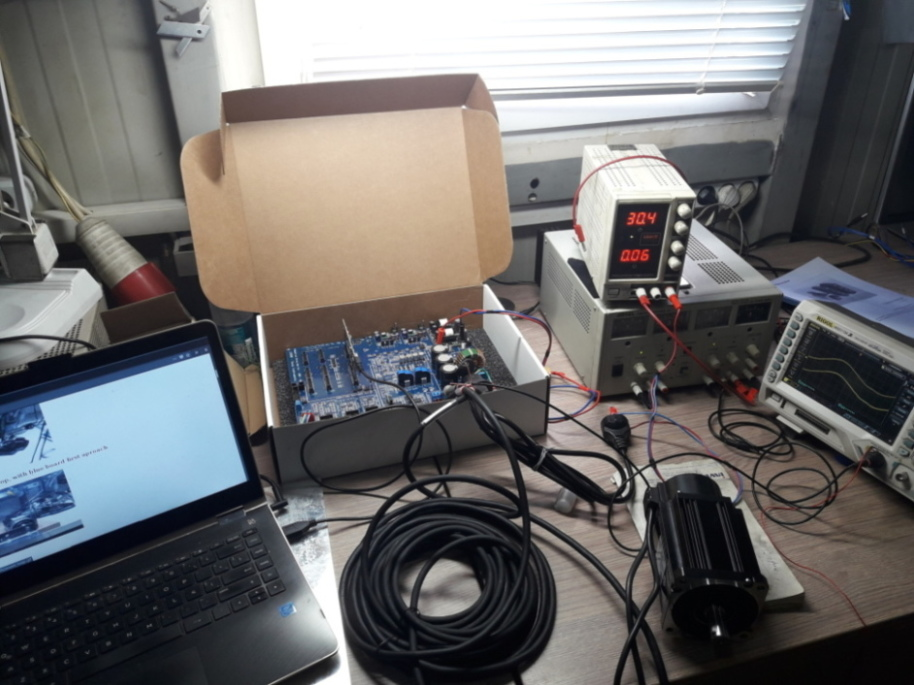
\includegraphics[width=0.3\textwidth]{nanocut1.jpg}
         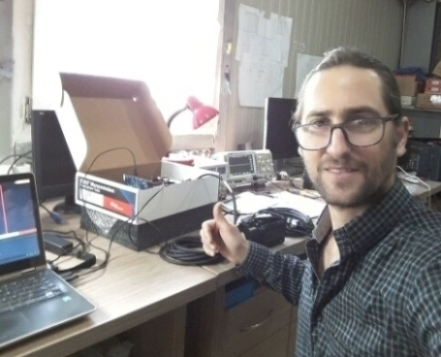
\includegraphics[width=0.3\textwidth]{nanocut2.jpg}
         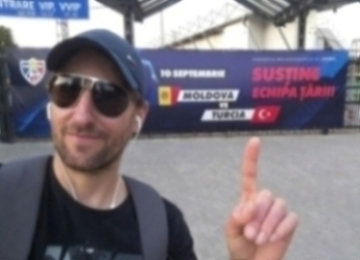
\includegraphics[width=0.3\textwidth]{nanocut3.jpg}
      \end{center}
      \caption{Development tools and algoritm output plots of the PMSM servo driver}
      \label{fig:nanocut_electronica}
   \end{figure}
   Figure \ref{fig:nanocut_mecanica} shows the prototype running at Nanocu's labs.
  \begin{figure}
      \begin{center}
         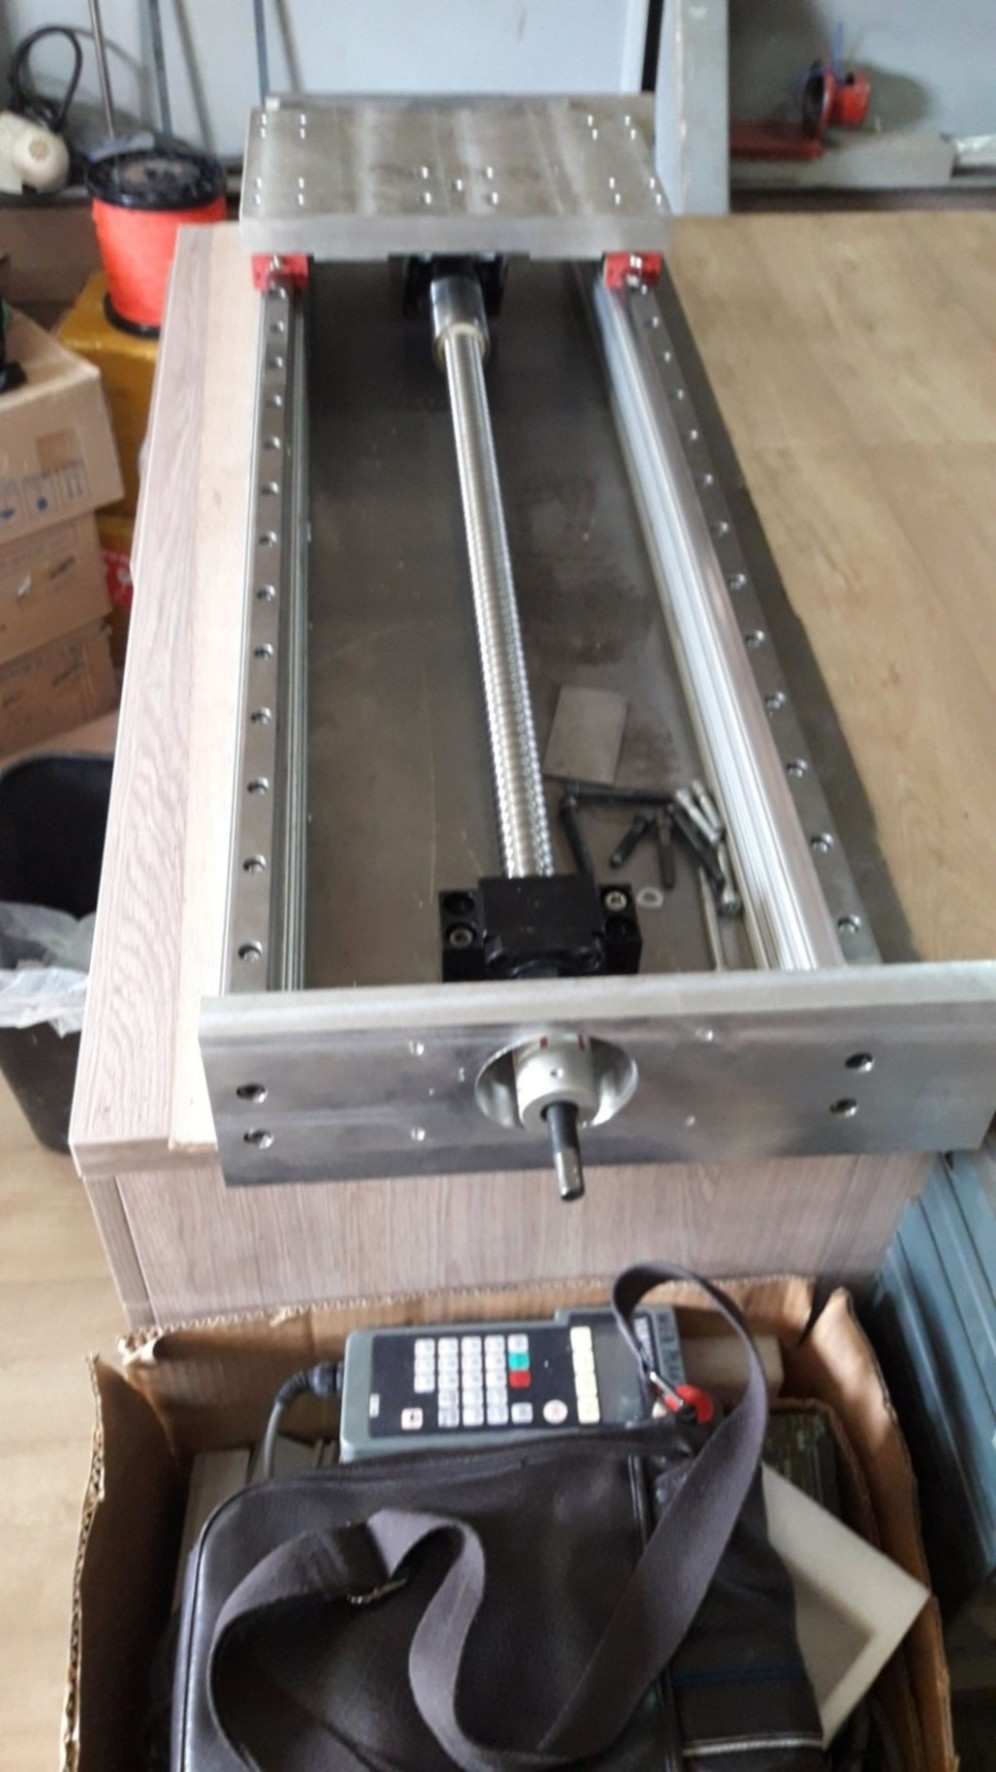
\includegraphics[width=0.3\textwidth]{nanocut4.jpg}
         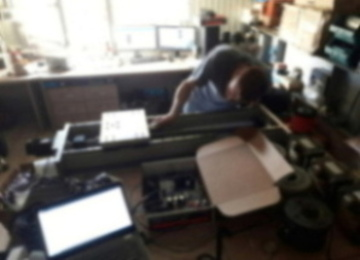
\includegraphics[width=0.3\textwidth]{nanocut5.jpg}
         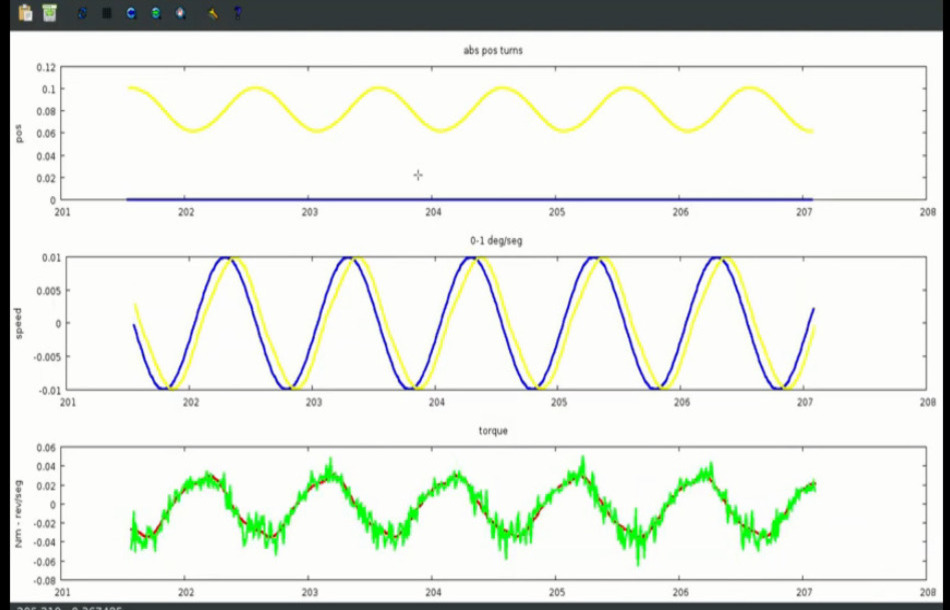
\includegraphics[width=0.3\textwidth]{nanocut6.jpg}
      \end{center}
      \caption{Mechanical prototype used for the PMSM algorithm test, torque, speed and position}
      \label{fig:nanocut_mecanica}
   \end{figure}

\subsection{\href{http://www.nanocut.com/}{Nanocut 3.0}}
   \hypertarget{subsec:nanocut}
   Working for Nanocut company at Moldova in first quarter of 2020 I've design the hardware for
   the new servo drive. I've made the schematics, layout routing and 3d model of the equipment.
   I've used Kicad 5.0 for all the process and complete the design using 6 layers traces of
   6mils/6mils, and vias of 0.3 mm min.
   There is the link of the public github project repository \href \linkgithubnanocutpcb {repo} and these is a video showing the final model \href {\linkgithubnanocutpcbvideoa} {video}.
   The board has the following main capacites:
   \begin{itemize}
      \item{Triple real time designed 32b 200MHz core procesar}
      \item{Differential isolated incremental encoder x2}
      \item{Differential isolated absolute encoder x2}
      \item{Differential isolated step direction input x2}
      \item{Isolated RS485 x1}
      \item{Isolated CAN x1}
      \item{Ethercat slave}
      \item{Ethernet}
      \item{Isolated current measurement using LEM x6}
      \item{Isolated voltage measurement x2}
      \item{Isolated PWM IGBT signals to x12}
      \item{Isolated alarm input x2}
      \item{Isolated brake output x2}
      \item{Isolated fan RMP measurement input x2}
      \item{Isolated sigma delta input x8}
      \item{Isolated NTC temperatura sensor x4}
      \item{Isolated 1-Wire bus x1}
      \item{SPI LCD interface for EVE touch screen modules or characters LCD plus}
      \item{Dual isolated power supply's}
      \item{Some others minor features}
   \end{itemize}

   With these capabilities the board could drive two PMSM motors at the same time and many
   powerful possibilities.  In the figure \ref{fig:nanocut_3_0_1} I show some pics of the design
   process.
  \begin{figure}
      \begin{center}
         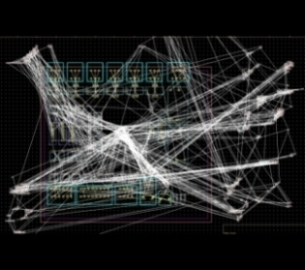
\includegraphics[width=0.3\textwidth]{nanocut_3_0_1.jpg}
         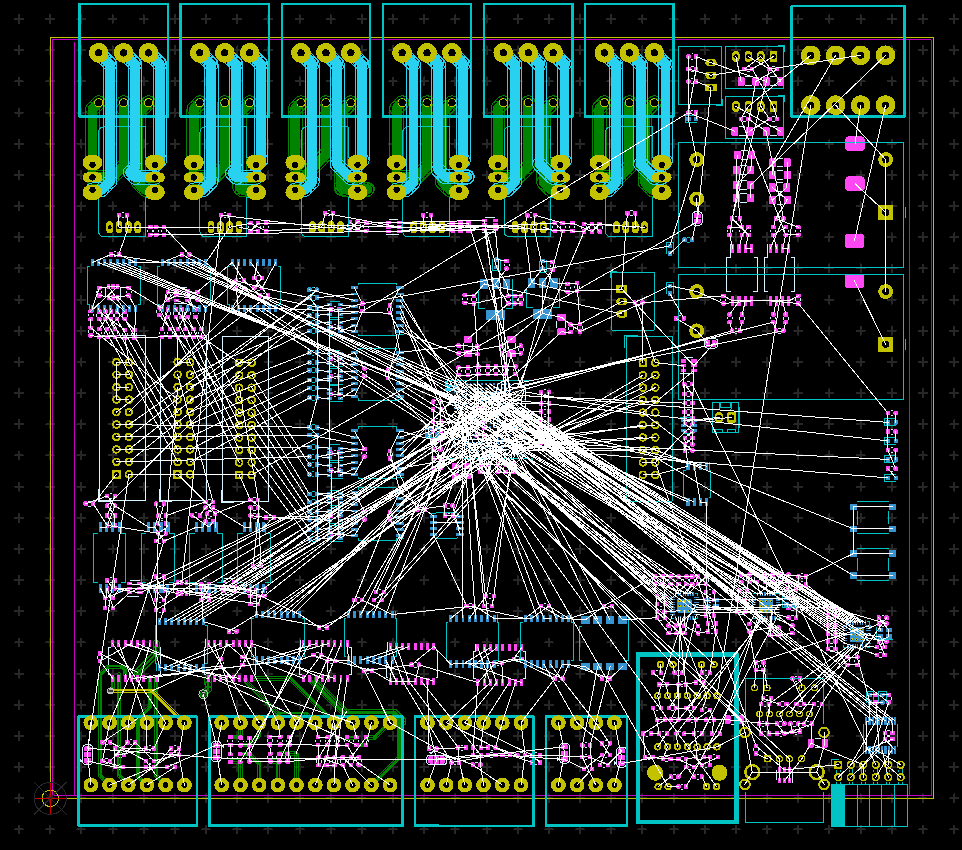
\includegraphics[width=0.3\textwidth]{nanocut_3_0_2.jpg}
         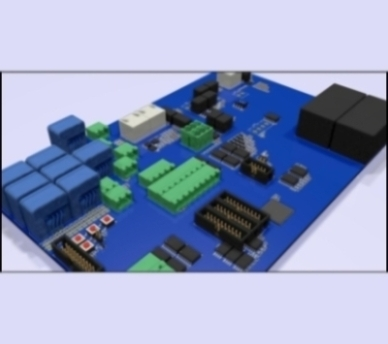
\includegraphics[width=0.3\textwidth]{nanocut_3_0_3.jpg}
      \end{center}
      \caption{PCB design stages at Nanocut Moldova for a PMSM servo drive.}
      \label{fig:nanocut_3_0_1}
   \end{figure}
In the figure \ref{fig:nanocut_3_0_2} I show some pics of the final release.
  \begin{figure}
      \begin{center}
         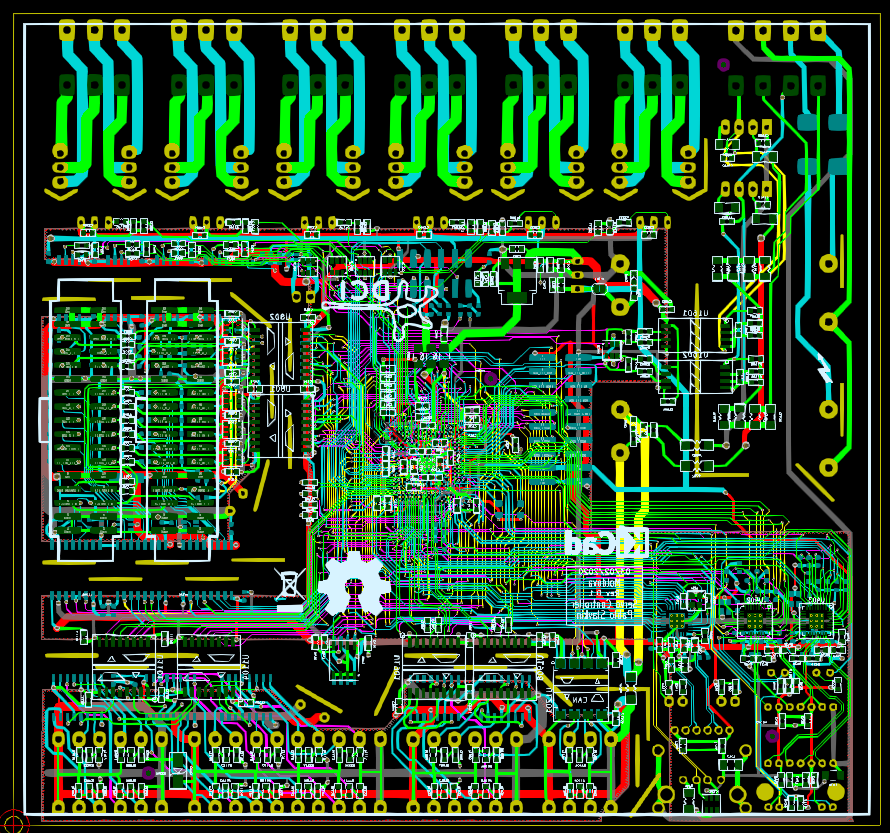
\includegraphics[width=0.3\textwidth]{nanocut_3_0_4.jpg}
         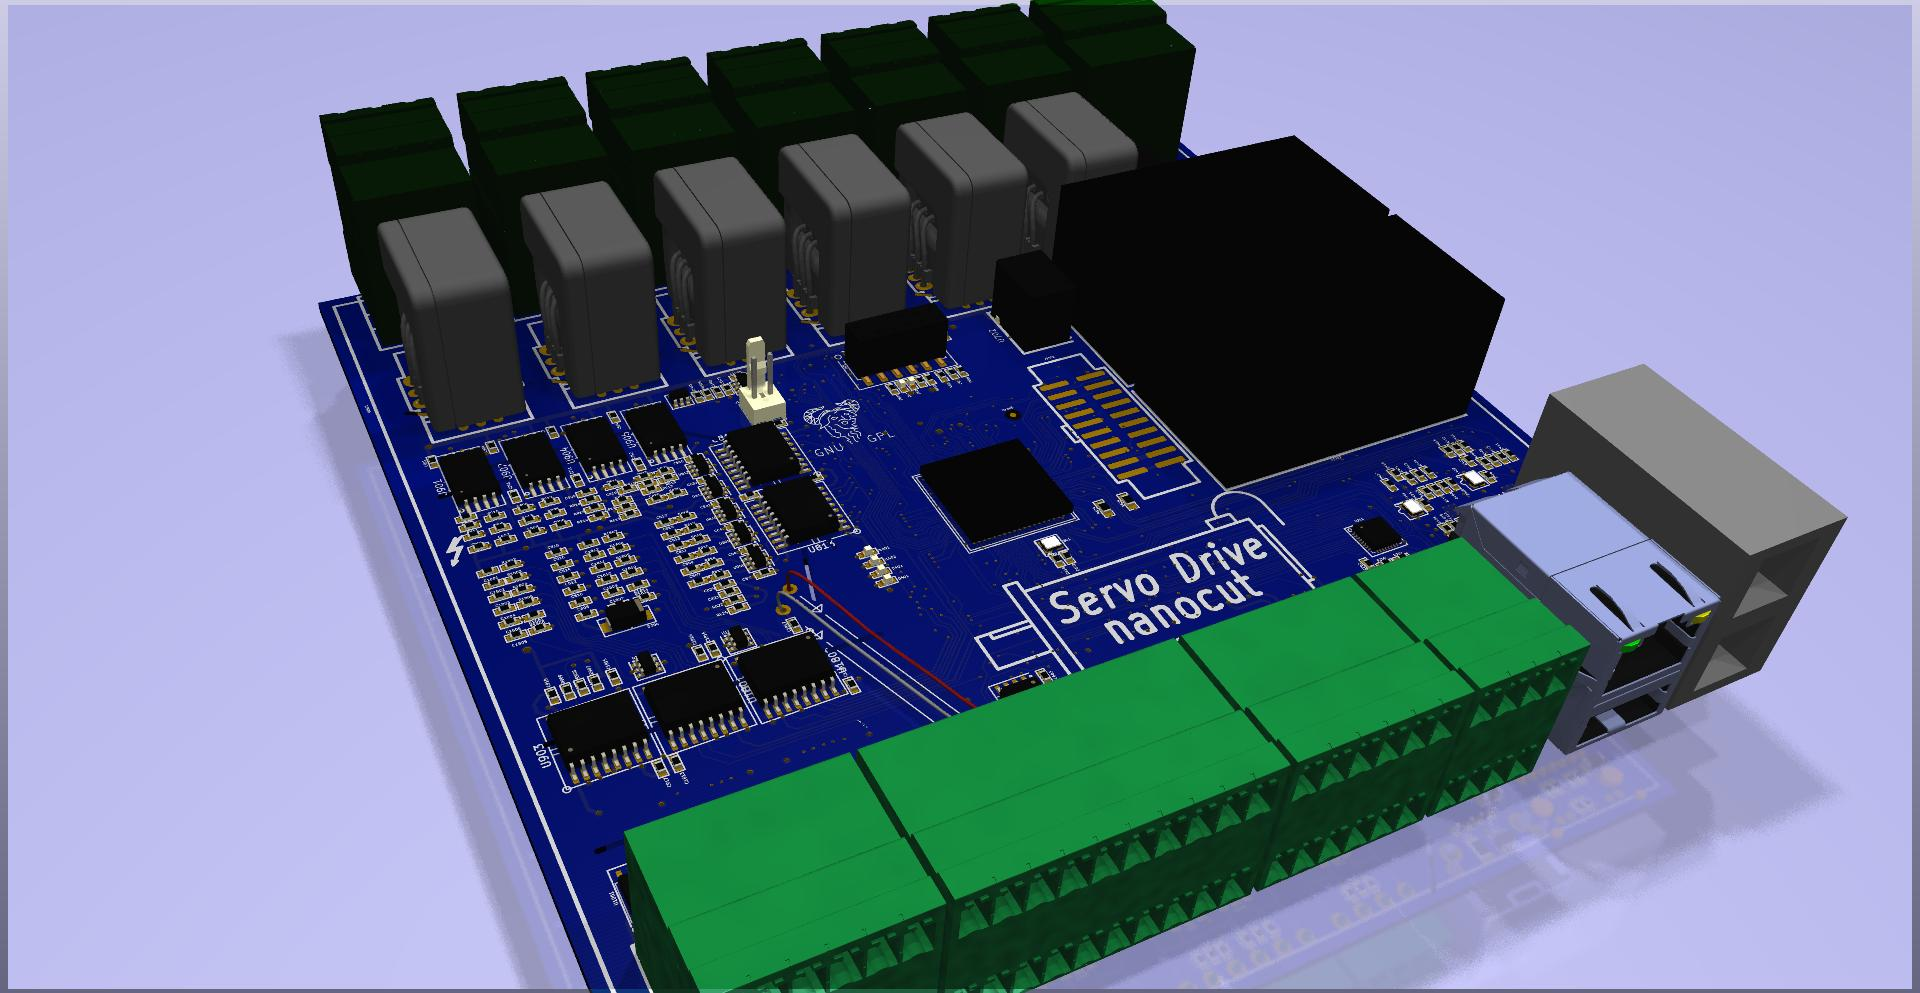
\includegraphics[width=0.3\textwidth]{nanocut_3_0_5.jpg}
         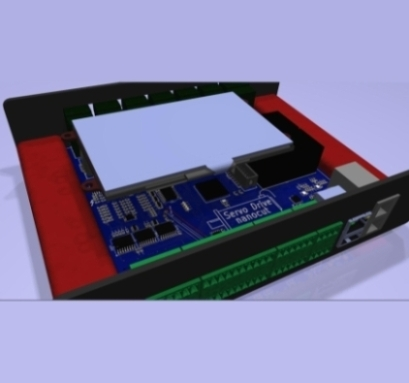
\includegraphics[width=0.3\textwidth]{nanocut_3_0_6.jpg}
      \end{center}
      \caption{PCB design release with a preliminary case at Nanocut Moldova for a PMSM servo drive.}
      \label{fig:nanocut_3_0_2}
   \end{figure}
